\documentclass[12pt,a4paper]{article}
\usepackage{graphicx}
\usepackage[utf8]{inputenc}
\usepackage{hyperref}
\usepackage{pgfplots}

\begin{document}
\begin{titlepage}
	\centering
	
\includegraphics[width=0.15\textwidth]{utec.png}\par\vspace{1cm}
	{\scshape\LARGE UTEC \par}
	\vspace{1cm}
	{\scshape\Large Reporte Unidad 6\par}
	\vspace{1.5cm}
	{\huge\bfseries Programacion orientada a objetos 2\par}
	\vspace{2cm}
	{\Large\itshape Alejandro Goicochea\par}
	\href{mailto:alejandro.goicochea@utec.edu.pe}{alejandro.goicochea@utec.edu.pe}
	\vfill
	Profesor:\par
	Ruben Rivas

	\vfill
	{\large \today\par}
\end{titlepage}

\section{Introducción}
En este ejercicio se estuvo trabajando con la programacion concurrente usando la libreria $<thread>$ de C++.
Se tiene como objetivo comparar el tiempo de ejecucion de la multiplicacion de dos matrices con dos clases diferentes.
Una tiene realiza la multiplicacion de manera secuencial y la otra de manera concurrente.

\section{Implementación}
Se crean dos clases $matriz\_reg$ y $matriz\_thread$ ambas con variables $n$ y $m$ que describen la cantidad 
de filas y columnas de su matriz, respectivamente. Ambas tambien cuentan con metodos para llenar su matriz de diferentes 
maneras. En el constructor de ambas se genera la matriz con los tama;os indicados en los parametros y se guarda en su variable 
matriz, un arreglo de tipo $int**$. Para la simplificacion del programa, se uso dos matrices del mismo tama;o (2000 x 2000) 
y el programa se ejecuto en un procesador Intel(R) Core(TM) i5-8250U CPU @ 1.60GHz con 8 threads. Para el benchmark se so la funcion
$clock()$ que mide el tiempo total del CPU. Este metodo para medir el tiempo considera el tiempo que tomo con todos los threads y devuelve 
el tiempo en la unidad $clock\_t$ por lo que dividimos nuestro resultado de $inicio$ - $fin$ por la cantidad de clocks por segundo almacenado 
en la variable $CLOCKS\_PER\_SEC$ multiplicado por la cantidad de threads que usamos (si la cantidad de threads usados es mayor a 8, se utiliza 
8 ya que el procesador en el que se ejecuto el programa solo tiene esa capacidad). El tiempo de ejecucion de la clase secuencial es el valor al ejecutar el 
programa con un solo thread.

\section{Resultados}
Al correr el programa el tiempo de ejecución empezó alto y fue bajando hasta llegar
a los 8 threads e incrementó nuevamente al agregar más llegando a un valor que parace ser asintotico.
\\

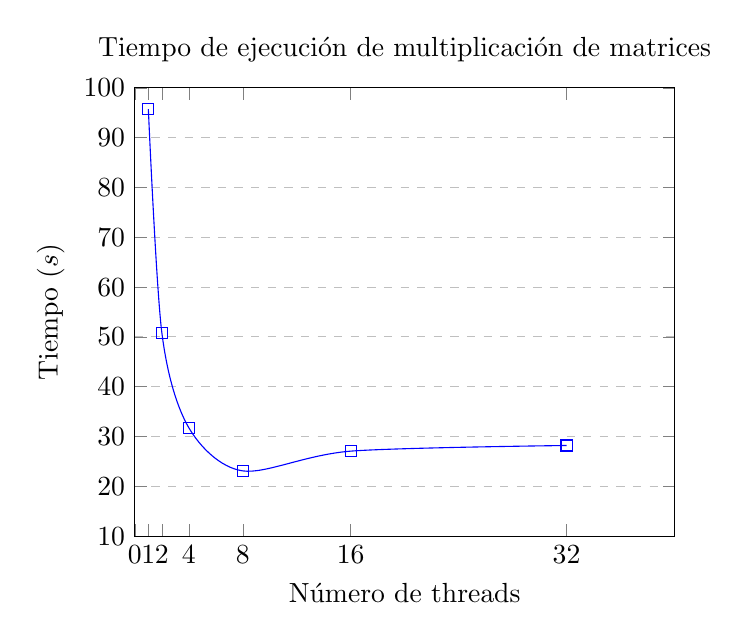
\begin{tikzpicture}
\begin{axis}[
    title={Tiempo de ejecución de multiplicación de matrices},
    xlabel={Número de threads},
    ylabel={Tiempo ($s$)},
    xmin=0, xmax=40,
    ymin=10, ymax=100,
    xtick={0,1,2,4,8,16,32},
    ytick={10,20,30,40,50,60,70,80,90,100},
    ymajorgrids=true,
    grid style=dashed,
]

\addplot[
    color=blue,
    mark=square,
		smooth
    ]
    coordinates {
    (1,95.7271)(2,50.8538)(4,31.7686)(8,23.107)(16,27.0718)(32,28.2049)
    };

\end{axis}
\end{tikzpicture}
\\
En este gráfico se ve claramente como el tiempo de ejecución baja hasta llegar a
los 8 threads y luego incrementa de nuevo llegando a una asíntota cercana a los 28 segundos.
De estos gráficos podemos concluir que el número óptimo de threads para nuestro programa va a ser
8 lo que coincide con el número de threads que tiene nuestro procesador. Es probable que el número óptimo de
threads que se debe crear en un programa sea igual a la cantidad de threads del procesador ya que si se crean más
threads de los que tiene el procesador van a haber threads esperando a que se libere otro thread del procesador. Si se crea
la cantidad de threads que tiene el procesador, se esta repartiendo las instrucciones del programa entre todos los threads
por lo que al terminar la ejecución de estos threads se termina la ejecución del programa ya que no había threads esperando
para ejecutarse.
\end{document}
